\documentclass[12pt,a4paper]{report}
\usepackage[utf8]{inputenc}
\usepackage{amsmath}
\usepackage{amsfonts}
\usepackage{amssymb}
\usepackage{graphicx}
\usepackage{commath}
\usepackage{array}
\usepackage{tabularx}
\usepackage{latexsym}
\usepackage[italian]{babel}
\usepackage{url} 
\usepackage{hyperref}
\usepackage[nottoc]{tocbibind}	
\usepackage[a4paper,top=1.5cm,bottom=1.8cm,left=1.5cm,right=1.5cm]{geometry}
\graphicspath{ {images/} }
\begin{document}
	\begin{titlepage}
		\begin{center}
	\huge{\textbf{Università della Calabria}}
	\begin{figure}[tb]
		\centering
		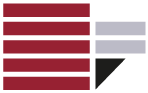
\includegraphics[scale=0.5]{logoUNICAL}
	\end{figure}
\end{center}
\begin{center}
	\line(1,0){400}\\[5mm]
	\Large{\textbf{Dipartimento di Matematica e Informatica}}
	\\\Large{\textbf{Corso di laurea in Informatica}}
	\\\vfill
	\Huge{\textbf{Data Warehouse Project \\\noindent CORDIS - EU research 2007-2013}}
	\vfill
\end{center}
\vfill
	\noindent \hfill  \Large{\text{Giovanni Brunetti}} \par
	\noindent \hfill	\Large{\textit{Matricola:}\text{193452}}
	\begin{center}
	\line(1,0){400}\\[5mm]
	{\large{\bf Anno accademico 2017/2018}}\\
\end{center}

	\end{titlepage}
\section*{Introduzione}
Lo scopo del progetto è quello di costruire un sistema di Data Warehouse basato sui dati relativi all'assegnazione di progetti scientifici da parte dell'UE alle varie organizzazioni mondiali.\\\noindent
Per far ciò si provvederà alla creazione del/dei data-mart necessari per i fatti di interesse in modo da permettere lo svolgersi delle analisi OLAP su di essi.
La progettazione ha seguito le varie fasi relativi all'approccio \textbf{source oriented}, includendo lo studio delle sorgenti, comprendendo operazioni di pulizia e di trasformazione dei dati per comprendere i dati ed il dominio di interesse. In seguito si è passato alla fase di alimentazione del database e dello studio dei dati ottenuti tramite analisi.\\\\\noindent
Per la fase di studio ,di ETL ed alimentazione del DB si è utilizzato il software Pentaho, mentre per lo studio dei dati e l'effettuazione delle analisi si è utilizzato il software Tableau.
\section*{Sorgente dei dati}
La sorgente dei dati è reperibile all' url  "https://data.europa.eu/euodp/data/dataset/cordisfp7projects" sotto forma di file csv.\\\noindent
La sorgente è composta da 6 file, essi contengono tutte le informazioni relativi ad ogni singolo progetto assegnato dal 2013 al 2017. La prima fase del progetto si è dunque concentrata nello studio di tutti i file per capire come essi erano connessi tra di loro. Essi infatti presentavano molte ripetizioni di attributi nei diversi file.
Per ciascuna delle assegnazioni le principali informazioni espresse e rilevanti del il data mart sono:
\begin{itemize}
	\item nome del progetto;
	\item le organizzazioni coinvolte nel progetto;
	\item la nazionalità di ogni organizzaione;
	\item programma di appartenenza del progettto;
	\item contributo economico dell'ue per ogni organizzazione;
	\item data di inizio e di fine.
\end{itemize}
\end{document}
\section*{Architettura di sistema}
L'architettura di sistema scelta per l'implementazione è quella a 3 livelli. Questa scelta è dovuta al fatto di avere più file come sorgente. Il 2 livello, ovvero quello dei dati riconciliati, permette di integrare le molteplici sorgenti per definire un unica fonte di dati operazionali. Così facendo si divide la fase di pulitura e di \textbf{ETL}, con la conseguente creazione delle dipendenze funzionali, da quello dell'alimentazione del Data Warehouse.
\begin{figure}[tb]
	\centering
	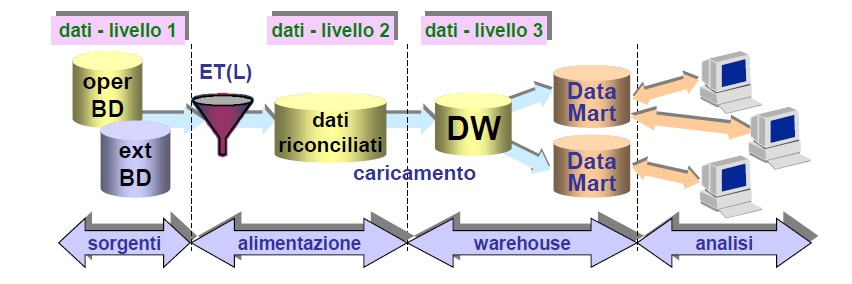
\includegraphics[scale=0.5]{architettura}
\end{figure}
